%% LyX 1.6.0 created this file.  For more info, see http://www.lyx.org/.
%% Do not edit unless you really know what you are doing.
\documentclass[10pt,english,trans]{beamer}
\usepackage{mathptmx}
\usepackage[T1]{fontenc}
\usepackage[latin9]{inputenc}
\usepackage{amsmath}
\usepackage{graphicx}
\usepackage{amssymb}

\makeatletter

%%%%%%%%%%%%%%%%%%%%%%%%%%%%%% LyX specific LaTeX commands.
%% A simple dot to overcome graphicx limitations
\newcommand{\notdot}{.}


%%%%%%%%%%%%%%%%%%%%%%%%%%%%%% Textclass specific LaTeX commands.
 % this default might be overridden by plain title style
 \newcommand\makebeamertitle{\frame{\maketitle}}%
 \AtBeginDocument{
   \let\origtableofcontents=\tableofcontents
   \def\tableofcontents{\@ifnextchar[{\origtableofcontents}{\gobbletableofcontents}}
   \def\gobbletableofcontents#1{\origtableofcontents}
 }
 \makeatletter
 \long\def\notframe#1{\@notframe#1\@notframestop}%
 \def\@notframe{\@ifnextchar<{\@@notframe}{\@@notframe<*>}}%
 \def\@@notframe<#1>{\@ifnextchar[{\@@@notframe<#1>}{\@@@notframe<#1>[]}}
 \def\@@@notframe<#1>[{\@ifnextchar<{\@@@@@notframe<#1>[}{\@@@@notframe<#1>[<*>][}}
 \def\@@@@@notframe<#1>[#2]{\@ifnextchar[{\@@@@notframe<#1>[#2]}{\@@@@notframe<#1>[#2][]}}
 \long\def\@@@@notframe<#1>[#2][#3]#4\@notframestop#5\notframeend{%
   \frame<#1>[#2][#3]{\frametitle{#4}#5}}
 \makeatother
 \newenvironment{centercolumns}{\begin{columns}[c]}{\end{columns}}
 \newenvironment{topcolumns}{\begin{columns}[t]}{\end{columns}}
\def\notframeend{} % In case there is a superfluous frame end

%%%%%%%%%%%%%%%%%%%%%%%%%%%%%% User specified LaTeX commands.
\usetheme{default}

%\usetheme[compress]{Ilmenau}
%\usetheme[left,width=2.0cm]{PaloAlto}
% or ...

\setbeamercovered{transparent}
% or whatever (possibly just delete it)
\usepackage{color}
% 
\xdefinecolor{JuelichBlau}{cmyk}{1.0,0.2,0.05,0.5}
\xdefinecolor{JuelichGruen}{cmyk}{0.23,0.0,1.0,0.17}
\xdefinecolor{JuelichGrau1}{cmyk}{0.0,0.0,0.0,0.80}
\xdefinecolor{JuelichGrau2}{cmyk}{0.0,0.0,0.0,0.50}
\xdefinecolor{JuelichGrau3}{cmyk}{0.0,0.0,0.0,0.30}

\setbeamercolor{palette primary}{fg=JuelichGruen,bg=JuelichGrau1}
\setbeamercolor{palette secondary}{bg=white}
\setbeamercolor{palette tertiary}{bg=JuelichGrau3}
\setbeamercolor{palette quaternary}{bg=JuelichGrau2}
%\setbeamercolor{titlelike}{bg=JuelichBlau}

\usecolortheme[named=JuelichBlau]{structure}

\useoutertheme[compress,footline=authortitle]{miniframes}
%\useoutertheme{shadow}
%\useoutertheme{infolines}

%\usefonttheme[onlylarge]{structurebold}

\makeatother

\usepackage{babel}


\begin{document}
\title{Dendritic growth in the presence of triple junctions and lattice strain: Green's function methods}

\author{C. H\"{u}ter}

\institute[]{Institute for Solid State Research, Theory of Structure Formation}


%\date{24th. June 2009}
\makebeamertitle

\logo{\vspace{9.0cm}\includegraphics[height=1.0cm]{Figures/logo_412.jpg}\hspace{0.5cm}}

%%%%%%%%%%%%%%%%%%%%%%%%%%%%%%%%%%%%%%%%%%%%%%%%%%%%%%%%%%%%%%%%%%%%%%%%
\section{}
\notframe{}

\tableofcontents{}


\notframeend{}
% %%%%%%%%%%%%%%%%%%%%%%%%%%%%%%%%%%%%%%%%%%%%%%%%%%%%%%%%%%%%%%%%%%%%%%%%
% %%%%%%%%%%%%%%%%%%%%%%%%%%%%%%%%%%%%%%%%%%%%%%%%%%%%%%%%%%%%%%%%%%%%%%%%
\section{Motivation and Introduction}
\notframe{Dendrites}
\begin{topcolumns}%{}
% 
% 
\column{5cm}
High-precision experiment to verify theoretical predictions:
\begin{figure}
\begin{centering}
\includegraphics[width=.71\textwidth]{Figures/xenonDendriteBilgram}
\par\end{centering}
\caption{Free single dendrite in Xenon, courtesy of J. Bilgram}
\end{figure}


\column{5cm}
Picture from standard industrial material:
\begin{figure}
\begin{centering}
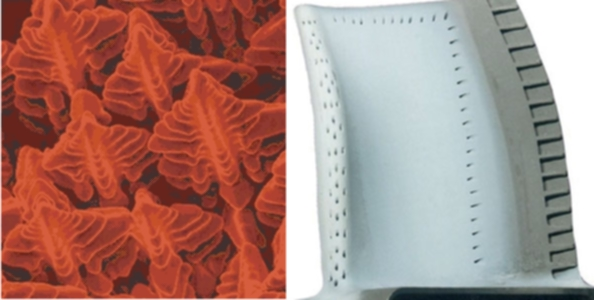
\includegraphics[width=1.15\textwidth]{Figures/dendriteArrayInBlade}
\par\end{centering}
\caption{Array of dendrites in Ni-based alloy, courtesy of ULTMAT}
\end{figure}
\end{topcolumns}

\begin{itemize}
\item fundamental pattern in metallurgical fabrication
\item understanding primary branch most important
\end{itemize}

\notframeend{}
%%%%%%%%%%%%%%%%%%%%%%%%%%%%%%%%%%%%%%%%%%%%%%%%%%%%%%%%%%%%%%%%%%%%%%%%
\notframe{}
\begin{topcolumns}%{}
% 
% 
\column{10cm}
\begin{figure}
\begin{centering}
\includegraphics[width=0.45\textwidth]{Figures/xenonDendritePrimaryBranchBilgram}
\par\end{centering}
\caption{The envelope indicates the primary Xenon branch.}
\end{figure}

\begin{itemize}
\item steady-state velocity $\upsilon$ of primary branch
%\item diffusion-limited growth 
%\item conservation law at moving interface
%\item local equilibrium 
\end{itemize}

\end{topcolumns}

\notframeend{}
%%%%%%%%%%%%%%%%%%%%%%%%%%%%%%%%%%%%%%%%%%%%%%%%%%%%%%%%%%%%%%%%%%%%%%%%
%\subsection{Diffusional transitions}
\notframe{Origin of growth: Mullins-Sekerka\\ vs. Gibbs-Thomson effect}
\begin{topcolumns}%{}
% 
% 
\column{5cm}
\begin{figure}
\begin{centering}
\includegraphics[width=.85\textwidth]{Figures/MS_bw_solidification}
\par\end{centering}
\caption{Mullins-Sekerka instability}
\end{figure}


\column{5cm}

\begin{figure}
\begin{centering}
\includegraphics[width=0.82\textwidth]{Figures/MSandGT_bw_solidification}
\par\end{centering}
\caption{Mullins-Sekerka instability vs  Gibbs-Thomson effect}
\end{figure}
\end{topcolumns}

\begin{itemize}
\item Mullins-Sekerka instability: lets protrusions grow further
\item Gibbs-Thomson effect counteracts: stabilizes interface shape 
%\item set Mullins-Sekerka length: $\lambda_{MS} \sim \sqrt{(d_0l_D)}$
%\item Mullins-Sekerka length is wavelength of maximal growth velocity

\end{itemize}

\notframeend{}

% %%%%%%%%%%%%%%%%%%%%%%%%%%%%%%%%%%%%%%%%%%%%%%%%%%%%%%%%%%%%%%%%%%%%%%%%
%\notframe{Diffusional transitions:\\ free or moving boundary problems}
\notframe{Diffusional transitions:\\ free or moving boundary problems}
\begin{topcolumns}%{}
% 
% 
\column{6cm}
\begin{itemize}
\item thermal diffusion:\footnote{$D$ diffusion constant}
\begin{eqnarray*}
D \nabla^2 T - \frac{\partial T}{\partial t} = 0 
\end{eqnarray*}

\item heat conservation:\footnote{$c_p$ heat capacity, $L$ latent heat}
\[\upsilon_n L= -c_p D \vec{n} \left( \nabla T_{m} - \nabla T_{s}  \right)\]
\item local equilibrium:\footnote{$\gamma$ surface energy, $T_M$ melting temperature, \\ ~~~~$\kappa$ curvature, $T_{|int}$ is $T$ at interface}
\[ T_{|int} = T_M - T_M \frac{\gamma\kappa}{L} \]

\end{itemize}

\column{5cm}
\begin{figure}
\begin{centering}
\includegraphics[width=0.80\textwidth]{Figures/selectionPic}
\par\end{centering}
\caption{The transition of the undercooled melt \begin{large}(m)\end{large} ($T_{\infty} \leq T_M$) to the solid phase \begin{large}(s)\end{large}}
\end{figure}

\end{topcolumns}



\notframeend{}
%%%%%%%%%%%%%%%%%%%%%%%%%%%%%%%%%%%%%%%%%%%%%%%%%%%%%%%%%%%%%%%%%%%%%%%%
%%%%%%%%%%%%%%%%%%%%%%%%%%%%%%%%%%%%%%%%%%%%%%%%%%%%%%%%%%%%%%%%%%%%%%%%
%\subsection{Green's function method}
\notframe{Green's function method}

\begin{topcolumns}%{}
% 
% 
\column{10cm}
\begin{itemize}
\item representation by \alert{boundary} integral equations:\footnote{$ {\cal{L}}[u] = D\nabla^2 u + \upsilon \frac{\partial u}{\partial y} = 0 $, $g:$ ${\cal L}_{\vec{x}}[g] = -\delta(\vec{x}-\vec{x}')$, ${\cal L}^{\dagger}_{\vec{x}'}[g] = -\delta(\vec{x}-\vec{x}')$}
\[ g{\cal{L}}[u] - u{\cal{L}}^{\dagger}[g] = \nabla J(u,g) \to - u{\cal{L}}^{\dagger}[g] = \nabla J(u,g)\] 
%\item experimental conditions: small undercoolings 
%\item approximated closed representation:\footnote{$A$ anisotropy, $\sigma$ stability parameter, $\kappa(\xi(x),x)$ curvature, $\xi(x)$ interface}
%\[ - A \sigma \kappa(\xi(x),x) = \int_{S'} f(x,\xi(x)|x',\xi(x')) \; ds' \]
\item thermodynamic identical domains ('symmetric model') \\ yield closed representation:\footnote{$\Delta = c_p (T_{eq}- T_\infty)/L$, $d_0 = c_p T_{eq} \gamma/L^2$, $p=\upsilon R/2D$, $R$ tip radius of asymptotically matching Ivantsov parabola}
\[ \Delta - A\frac{d_0 \kappa}{R} = 2p \int_S g \; ds \]
\item nonlinear integro-differential \alert{interface} equation
% \item $A = 1$, isotropic surface tension: no steady state solution
% \item $A$ anisotropic: discrete spectrum of selected solutions
% \item $\Delta \ll 1$: $\sigma = d_0/pR$ const, velocity:\footnote{$\Delta \leq 1$ undercooling}  $\upsilon \sim \sigma \Delta^4$ 
%\item unique growth direction along maximal surface tension
\end{itemize}

\end{topcolumns}


\notframeend{}
%%%%%%%%%%%%%%%%%%%%%%%%%%%%%%%%%%%%%%%%%%%%%%%%%%%%%%%%%%%%%%%%%%%%%%%%
%\subsection{Green's function method}
\notframe{Finding new stationary growth mechanisms}
\begin{topcolumns}%{}
% 
% 
\column{10cm}
\[ \Delta - A\frac{d_0 \kappa}{R} = 2p \int_S g \; ds\]


\begin{itemize}
%\item dimesion of problem reduced
%\item $A = 1$, isotropic surface tension: no steady state solution
%\item $A$ anisotropic: discrete spectrum of selected solutions
\item $\Delta \ll 1$: $\sigma = \frac{d_0 l_D}{R^2}$\footnote{$R$ characteristic lengthscale, $l_D=2D/\upsilon$, $\Delta = c_p (T_{eq}- T_\infty)/L$, $d_0 = c_p T_{eq} \gamma/L^2$, $p=\upsilon R/2D$} const, velocity: $\upsilon \sim \sigma \Delta^4$  %\footnote{$\Delta \leq 1$ undercooling}
%\item \begin{large} $A=1 \quad \& \quad \sigma \neq 0$: new selection mechanism \end{large}
\end{itemize}

%\begin{large} $A=1 \quad \& \quad \sigma \neq 0$: new selection mechanism \end{large}

\end{topcolumns}

\notframeend{}
%%%%%%%%%%%%%%%%%%%%%%%%%%%%%%%%%%%%%%%%%%%%%%%%%%%%%%%%%%%%%%%%%%%%%%%%
%%%%%%%%%%%%%%%%%%%%%%%%%%%%%%%%%%%%%%%%%%%%%%%%%%%%%%%%%%%%%%%%%%%%%%%%
%\subsection{Green's function method}
\notframe{Finding new stationary growth mechanisms}
\begin{topcolumns}%{}
% 
% 
\column{10cm}
\[ \Delta - A\frac{d_0 \kappa}{R} = 2p \int_S g \; ds\]


\begin{itemize}
%\item dimesion of problem reduced
% \item $\Delta \ll 1$: $\sigma = d_0/pR$\footnote{$\Delta = c_p (T_{eq}- T_\infty)/L$, $d_0 = c_p T_{eq} \gamma/L^2$, $p=\upsilon R/2D$} const, velocity: $\upsilon \sim \sigma \Delta^4$  %\footnote{$\Delta \leq 1$ undercooling}
\item $\Delta \ll 1$: $\sigma = \frac{d_0 l_D}{R^2}$\footnote{$R$ characteristic lengthscale, $l_D=2D/\upsilon$, $\Delta = c_p (T_{eq}- T_\infty)/L$, $d_0 = c_p T_{eq} \gamma/L^2$, $p=\upsilon R/2D$} const, velocity: $\upsilon \sim \sigma \Delta^4$
\item $A = 1$, isotropic surface tension: no stationary solution
%\item $A$ anisotropic: discrete spectrum of selected solutions
%\item \begin{large} $A=1 \quad \& \quad \sigma \neq 0$: new selection mechanism \end{large}
\end{itemize}

%\begin{large} $A=1 \quad \& \quad \sigma \neq 0$: new selection mechanism \end{large}

\end{topcolumns}

\notframeend{}
%%%%%%%%%%%%%%%%%%%%%%%%%%%%%%%%%%%%%%%%%%%%%%%%%%%%%%%%%%%%%%%%%%%%%%%%
%%%%%%%%%%%%%%%%%%%%%%%%%%%%%%%%%%%%%%%%%%%%%%%%%%%%%%%%%%%%%%%%%%%%%%%%
%\subsection{Green's function method}
\notframe{Finding new stationary growth mechanisms}
\begin{topcolumns}%{}
% 
% 
\column{10cm}
\[ \Delta - A\frac{d_0 \kappa}{R} = 2p \int_S g \; ds\]


\begin{itemize}
%\item dimesion of problem reduced
\item $\Delta \ll 1$: $\sigma = \frac{d_0 l_D}{R^2}$\footnote{$R$ characteristic lengthscale, $l_D=2D/\upsilon$, $\Delta = c_p (T_{eq}- T_\infty)/L$, $d_0 = c_p T_{eq} \gamma/L^2$, $p=\upsilon R/2D$} const, velocity: $\upsilon \sim \sigma \Delta^4$
% \item $\Delta \ll 1$: $\sigma = d_0/pR$\footnote{$\Delta = c_p (T_{eq}- T_\infty)/L$, $d_0 = c_p T_{eq} \gamma/L^2$, $p=\upsilon R/2D$} const, velocity: $\upsilon \sim \sigma \Delta^4$  %\footnote{$\Delta \leq 1$ undercooling}
\item $A$ anisotropic: discrete spectrum of solutions
%\item $A = 1$, isotropic surface tension: no steady state solution
%\item \begin{large} $A=1 \quad \& \quad \sigma \neq 0$: new selection mechanism \end{large}
\end{itemize}

%\begin{large} $A=1 \quad \& \quad \sigma \neq 0$: new selection mechanism \end{large}

\end{topcolumns}

\notframeend{}
%%%%%%%%%%%%%%%%%%%%%%%%%%%%%%%%%%%%%%%%%%%%%%%%%%%%%%%%%%%%%%%%%%%%%%%%
%%%%%%%%%%%%%%%%%%%%%%%%%%%%%%%%%%%%%%%%%%%%%%%%%%%%%%%%%%%%%%%%%%%%%%%%
%\subsection{Green's function method}
\notframe{Finding new stationary growth mechanisms}
\begin{topcolumns}%{}
% 
% 
\column{10cm}
\[ \Delta - A\frac{d_0 \kappa}{R} = 2p \int_S g \; ds\]


\begin{itemize}
%\item dimesion of problem reduced
%\item $\Delta \ll 1$: $\sigma = d_0/pR$\footnote{$\Delta = c_p (T_{eq}- T_\infty)/L$, $d_0 = c_p T_{eq} \gamma/L^2$, $p=\upsilon R/2D$} const, velocity: $\upsilon \sim \sigma \Delta^4$  %\footnote{$\Delta \leq 1$ undercooling}
\item $\Delta \ll 1$: $\sigma = \frac{d_0 l_D}{R^2}$\footnote{$R$ characteristic lengthscale, $l_D=2D/\upsilon$, $\Delta = c_p (T_{eq}- T_\infty)/L$, $d_0 = c_p T_{eq} \gamma/L^2$, $p=\upsilon R/2D$} const, velocity: $\upsilon \sim \sigma \Delta^4$
\item $A = 1$, isotropic surface tension: no steady state solution
\item $A$ anisotropic: discrete spectrum of solutions
\item \begin{large} Are there other effects which lead to new stationary growth with isotropic surface tension ? \end{large}
%\item \begin{large} \alert{$A=1 \quad \& \quad \sigma \neq 0$: new selection mechanism} \end{large}
\end{itemize}

%\begin{large} $A=1 \quad \& \quad \sigma \neq 0$: new selection mechanism \end{large}

\end{topcolumns}

\notframeend{}
%%%%%%%%%%%%%%%%%%%%%%%%%%%%%%%%%%%%%%%%%%%%%%%%%%%%%%%%%%%%%%%%%%%%%%%%
%%%%%%%%%%%%%%%%%%%%%%%%%%%%%%%%%%%%%%%%%%%%%%%%%%%%%%%%%%%%%%%%%%%%%%%%
%\subsection{Dendritic growth and selection}
\notframe{Solved systems \& Focus}

\begin{itemize}
 \item thermal diffusional transitions subjected to lattice strain
\begin{itemize}
%\item single crystal dilatation/ shear
%\item single crystal shear 
\item \begin{large} \alert{single crystal shear+dilatation} \end{large}
\item single crystal zero elastic hysteresis
%\item bicrystal shear
\item bicrystal shear+dilatation 
%\item bicrystal regular triple junction
\item bicrystal pure elastically induced stationary growth
\end{itemize}
\end{itemize}
\begin{itemize}
\item chemical diffusional transitions at triple junctions
\begin{itemize}
\item isolated eutectoid dendrite 
\item \alert{asymmetric monotectic dendrite}  
\end{itemize}
\end{itemize}




\notframeend{}
% %%%%%%%%%%%%%%%%%%%%%%%%%%%%%%%%%%%%%%%%%%%%%%%%%%%%%%%%%%%%%%%%%%%%%%%%
%%%%%%%%%%%%%%%%%%%%%%%%%%%%%%%%%%%%%%%%%%%%%%%%%%%%%%%%%%%%%%%%%%%%%%%%
\section{Elasticity-induced stationary growth}
\notframe{Solid-solid transitions limited by\\ diffusion of latent heat: influence of lattice strain}
Elastic effects (structure transitions, density variations) present in various solid-solid transitions
\begin{figure}
\begin{centering}
\includegraphics[width=0.30\textwidth]{Figures/widmanStaettenLarge}
\par\end{centering}
\caption{Widmanstaetten plates in $Fe-C$ alloy. Scale $\sim$ 100 $\mu m$, courtesy of N. Stanford}
\end{figure}
\begin{itemize}
\item diffusional and elastic model
%\item elastic model
\item closed representation and stationary growth 
\item solution of single crystal configurations
%\item (applications in bicrystal geometry)
%\item (zero velocity and zero hysteresis)
\end{itemize}

\notframeend{}
% %%%%%%%%%%%%%%%%%%%%%%%%%%%%%%%%%%%%%%%%%%%%%%%%%%%%%%%%%%%%%%%%%%%%%%%%
%\subsection{Model}
% \framesubtitle{single crystal}

%%%%%%%%%%%%%%%%%%%%%%%%%%%%%%%%%%%%%%%%%%%%%%%%%%%%%%%%%%%%%%%%%%%%%%%
% 
%\section{Diffusional model} 
\notframe{Diffusional model}
\begin{topcolumns}%{}
% 
% 
\column{10cm}
\begin{itemize}
\item thermal diffusion%:\footnote{$w = c_p (T - T_\infty)/L$, $c_p$ heat capacity, \\~~~~~$L$ latent heat, $l_D=2D/\upsilon$ diffusion length}%
 %\\ ~~~~$\nabla^2 w + \frac{2}{l_D} \frac{\partial w}{\partial y} = 0$%
% \begin{eqnarray*}
% \nabla^2 w + \frac{2}{l_D} \frac{\partial w}{\partial y} = 0 
% \end{eqnarray*}
\end{itemize}
\begin{itemize}
%\footnote{$c_p$ heat capacity,$L$ latent heat,\\~~~~ $l_D=2D/\upsilon$ diffusion length} 
\item heat conservation%:\footnote{$D$ th. diffusion coefficient}
%\[\upsilon_n = D \vec{n} \left( \nabla w_{\beta} - \nabla w_{\alpha}  \right)\]
% \\ ~~~~$\upsilon_n = D \vec{n} \left( \nabla w_{\beta} - \nabla w_{\alpha}  \right)$%
\end{itemize}
\begin{itemize}
\item local equilibrium(\alert{+elastic effects}):\footnote{$\Delta = c_p (T_{eq}- T_\infty)/L$, $d = c_p T_{eq} \gamma/L^2$, \\~~~~~$\gamma$ surface energy, $w = c_p (T - T_\infty)/L$, $c_p$ heat capacity, \\~~~~~$L$ latent heat} 
\[ w_{|int} = \Delta - d \kappa + \alert{T_{eq} c_p \delta \tilde{F}^{el} /L^2 }\]
% \\ ~~~~$w_{|int} = \Delta - d \kappa + T_{eq} c_p \delta \tilde{F}^{el} /L^2$%
% \item $\Delta = c_p (T_{eq}- T_\infty)/L$%
% \item $d = c_p T_{eq} \gamma/L^2$%
\end{itemize}
\begin{itemize}
\item reduced thermal-elastic coupling 
% \item %
% \footnote{}
% \item %
% \footnote{}

\end{itemize}
% 
\end{topcolumns}
% 
\notframeend{}
% %%%%%%%%%%%%%%%%%%%%%%%%%%%%%%%%%%%%%%%%%%%%%%%%%%%%%%%%%%%%%%%%%%%%%%%%
\notframe{Elastic Model}

\begin{centercolumns}
\column{5.0cm}
\begin{itemize}
%\item Motivation: 
% \item Linear isotropic elasticity
% \item Symmetry of phases: $E^{(\alpha)}=E^{(\beta)}$,$\nu^{(\alpha)}=\nu^{(\beta)}$%
%  \footnote{$E$ elastic modulus, $\nu$ Poisson ratio} 
\item coherency\footnote{Displacements $ \vec{u}$}: $ \vec{u}^{(\alpha)} = \vec{u}^{(\beta)} $
\item elastic free energy\footnote{$\epsilon_{ik}=\left(\partial_{x_{k}}u_{i}+\partial_{x_{i}}u_{k}\right)/2$,\\$\sigma_{ik}=E/(1+\nu) (\epsilon_{ik}+\nu/(1-2\nu) \delta_{ik} \epsilon_{ik})$}%
\begin{eqnarray*}
%$\vec{u}$}: $\vec{u}^{(\alpha)} = \vec{u}^{(\beta)}$%
% \item Solid-solid phase transitions $\to$ lattice strains $\epsilon^0_{ik}$
% %$F_{el}^{(\beta)} = 1/2 \; \sigma_{ik} (\epsilon_{ik} - \epsilon^0_{ik})$
F_{el}^{(\beta)} &=& \frac{1}{2} \sigma_{ik} \epsilon^{(\beta)}_{ik} \\
%F_{el}^{(\beta)} &=& \frac{1}{2} \sigma_{ik} (\epsilon_{ik} - \epsilon^0_{ik}) \\
F_{el}^{(\alpha)} &=& \frac{1}{2} \sigma_{ik} \epsilon^{(\alpha)}_{ik}\\
%\footnote{}
% %$\delta \tilde{F}^{el} = \tilde{F}^{el}_{(\alpha)}-\tilde{F}^{el}_{(\beta)}$%
\delta \tilde{F}^{el} &=& \tilde{F}^{el}_{(\alpha)}-\tilde{F}^{el}_{(\beta)}%
\end{eqnarray*}
% \footnote{$\tilde{F}^{el} = F^{el} -\sigma_{nn}\epsilon_{nn}-2\sigma_{n\tau}\epsilon_{n\tau}$}
% %\item Plain strain%
% %\item $F_{el}^{(\beta)} = \frac{E}{2(1-\nu)} \left( \frac{\nu}{1-2\nu} (\epsilon_{ii} - \epsilon^0_{ii})^2  + (\epsilon_{ik}-\epsilon^0_{ik})^2 \right) $
\end{itemize}


\column{5cm}
% 
% %
\begin{figure}
\begin{centering}
\includegraphics[width=0.65\textwidth]{Figures/EigenstrainDilat}
\par\end{centering}
%,height=50pt
\caption{Coherent interface with eigenstrain $\epsilon^0_{ik} = \delta_{ik}\epsilon$}
\begin{centering}
\includegraphics[width=0.8\textwidth]{Figures/HexagonalToOrthorombic2}
\par\end{centering}
\caption{Transition from hexagonal to orthorhombic hexagonal structure}
\end{figure}
% 
\end{centercolumns}
\notframeend{}

% %%%%%%%%%%%%%%%%%%%%%%%%%%%%%%%%%%%%%%%%%%%%%%%%%%%%%%%%%%%%%%%%%%%%%%%%
% 
% 
%\section{Closed representation}
\notframe{Closed representation}
\begin{topcolumns}

\column{12cm}
\begin{itemize}
%\item eliminate both - temperature $w$ and strains $\epsilon_{ik}$: 
\item closed representation as interface equation:\footnote{$\delta\tilde{F}^{el} = \delta\tilde{F}^{el}[\epsilon_{ik}(\vec{x})]$, $g(\vec{x},\vec{x}\;') = 1/2\pi \;\;\; e^{-p(y-y\;')} \mathit{K}_0(p\eta(\vec{x}, \vec{x}\;')) $,\\ $\eta(\vec{x}, \vec{x}\;') = \| \vec{x}-\vec{x}\;'\|$, $p = \upsilon R/2D$, $R$ is radius of asymptotically matching Ivantsov parabola}
\end{itemize}

% $\Delta - d \kappa/R + T_{eq} c_p \delta \tilde{F}^{el}[\epsilon_{ik}(\vec{x},\vec{x}\;')]/L^2 =$ 
%  ~~~~$ p/\pi \int_{-\infty}^{\infty} dx' \exp[-p(y(x)-y(x'))] K_0(p \eta(x, x'))$%
%\begin{align}
\[ \Delta - \frac{d_0 \kappa}R + \alert{\frac{T_{eq} c_p \delta \tilde{F}^{el}}{L^2}} =  2p\int_{-\infty}^{\infty} dx' g(\vec{x},\vec{x}\;')\]%
%\end{align}%



%\begin{itemize}
%\item $p \ll 1$:\footnote{$\Delta_{el} \sim c_p T_{eq} E \epsilon^2 /L^2$: asymptotic shift of interface temperature by elastic effects} remaining control parameter $\Delta_{el}/p$%, eigenvalue $\sigma = d_0/pR$
%\end{itemize}
\begin{itemize}
\item stationary growth: \alert{$\sigma \neq 0$}\footnote{$\sigma = d_0/pR$} for smooth tip $\to \upsilon \sim \sigma \tilde{\Delta}^4$ 
% \item closed representation as interface equation
% \item elastic hysteresis: \\
% \begin{itemize}
% 	\item $\tilde{\Delta} = \Delta - \Delta_{el}$%
% 	\item $\tilde{\Delta} = (\pi p)^{1/2} \mathit{e}^p \mathit{erfc}(p^{1/2})$ 
% \end{itemize}
\end{itemize}

\end{topcolumns}
\notframeend{}
% 
% %%%%%%%%%%%%%%%%%%%%%%%%%%%%%%%%%%%%%%%%%%%%%%%%%%%%%%%%%%%%%%%%%%%%%%%%
%\subsection{Applied Configurations}
\notframe{Single Crystal}
\begin{topcolumns}
% 
% 
\column{6cm}
\begin{itemize}
\item pure dilatation/shear: no stationary growth

\end{itemize}
%$(\epsilon^0)^d_{ik}=\delta_{ik}\epsilon$, $(\epsilon^0)^s_{xx}= -\epsilon \cos 2\vartheta$,$(\epsilon^0)^s_{yy}= \epsilon \cos 2\vartheta$,$(\epsilon^0)^s_{xy}= \epsilon \sin 2\vartheta$ | single Crystal $\to$ $\vartheta = 0$


 
\column{6cm}
\begin{itemize}
% \item pure dilatation/shear: analytically/numerically absence of selection
% \item pure : numerically absence of solution
%\item superposition:%\footnote{$(\epsilon^0)^d= 
% \left( \begin{array}{ccc}
% 1 & 0 & 0 \\
% 0 & 1 & 0 \\						
% 0 & 0 & 1 	
% \end{array} \right)$, \\ 
% ~~~~~$(\epsilon^0)^s =
% \left( \begin{array}{ccc}
% -1 & 0 & 0 \\
% 0 & 1 & 0 \\						
% 0 & 0 & 0 	
% \end{array} \right)$}
%$(\epsilon^0)^{\pm}_{ik} = \eta (\epsilon^0)^d_{ik}\pm(1-\eta)(\epsilon^0)^s_{ik}$%

\item $(\epsilon^0)^-$ grows, $(\epsilon^0)^+$ not %\\
%preferred mode: largest deformation $\perp$ growth direction
\item magnitudes up to $\sigma \sim 10$
\end{itemize}
% \begin{figure}
% % \begin{centering}
% % \includegraphics[width=0.7\textwidth]{Figures/sC_sOfdeltaEl_01_03_05_mod}
% % \par\end{centering}
% % \caption{$\sigma(\Delta_{el}/p)$ for varying $\eta$}
% \begin{centering}
% \includegraphics[width=0.9\textwidth]{Figures/sC_sOfEta_deltaEl_1_mod}
% \par\end{centering}
% \caption{$\sigma$ for varying $\eta$, $\Delta_{el}/p=1$}
% \end{figure}

\end{topcolumns}%{}
% 
\begin{figure}
\begin{centering}
%\includegraphics[width=0.92\textwidth]{Figures/sC_sOfdeltaEl_01_03_05_mod}
\includegraphics[width=1.0\textwidth]{Figures/sCBoth}
\par\end{centering}
\caption{$\sigma(\Delta_{el}/p)$ for varying $\eta$, $\sigma$ for varying $\eta$, $\Delta_{el}/p=1$}
\end{figure}
\notframeend{}
% 

% %%%%%%%%%%%%%%%%%%%%%%%%%%%%%%%%%%%%%%%%%%%%%%%%%%%%%%%%%%%%%%%%%%%%%%%%
%\section{Summary and Outlook}
\notframe{Summary}
\begin{itemize}
\item model for closed representation of elastic-diffusional phase transition
\end{itemize}
\begin{itemize}
\item lattice strains can lead to stationary growth with isotropic surface tension
\end{itemize}
\begin{itemize}
\item larger growth velocities $\sigma \sim 10$ than in classical dendritic growth
\end{itemize}
\begin{itemize}
\item growth velocity depends on relative orientation of lattice strain and growth direction 
\end{itemize}
%\item results supported by phasefield simulations, dynamically stable
% \item solution of bicrystal geometries
% \item calculations for asymptotic regime $\Delta_{el}/p \ll 1$
% \item calculations for vanishing elastic hysteresis $\Delta_{el} = 0$
\notframeend{}
% %%%%%%%%%%%%%%%%%%%%%%%%%%%%%%%%%%%%%%%%%%%%%%%%%%%%%%%%%%%%%%%%%%%%%%%%
\notframe{Solved systems \& Focus}

\begin{itemize}
 \item thermal diffusional transitions subjected to lattice strain
\begin{itemize}
%\item single crystal dilatation/ shear
%\item single crystal shear 
\item \alert{single crystal shear+dilatation}
\item single crystal zero elastic hysteresis
%\item bicrystal shear
\item bicrystal shear+dilatation 
%\item bicrystal regular triple junction
\item bicrystal pure elastically induced stationary growth
\end{itemize}
\end{itemize}
\begin{itemize}
\item chemical diffusional transitions at triple junctions
\begin{itemize}
\item isolated eutectoid dendrite 
\item \begin{large} \alert{asymmetric monotectic dendrite} \end{large} 
\end{itemize}
\end{itemize}




\notframeend{}
% %%%%%%%%%%%%%%%%%%%%%%%%%%%%%%%%%%%%%%%%%%%%%%%%%%%%%%%%%%%%%%%%%%%%%%%%
%%%%%%%%%%%%%%%%%%%%%%%%%%%%%%%%%%%%%%%%%%%%%%%%%%%%%%%%%%%%%%%%%%%%%%%%
\section{Stationary growth at triple junctions}
\notframe{Chemical diffusional transitions:\\ influence of a triple junction}

\begin{figure}
\begin{centering}
\includegraphics[width=0.60\textwidth]{Figures/monotecticDendrite2}
\par\end{centering}
\caption{Cu-Nb dendrites, Scale $\sim 10 \mu m$ }
\end{figure} 

% {\large{eutectoid transition}} 
% \begin{itemize}
% \item geometry and symmetric model
% \item results 
% \end{itemize}
{\large{monotectic transition}}
\begin{itemize}
\item the one-sided liquid-liquid symmetric model
\item results  
\end{itemize}

\notframeend{}
% %%%%%%%%%%%%%%%%%%%%%%%%%%%%%%%%%%%%%%%%%%%%%%%%%%%%%%%%%%%%%%%%%%%%%%%%

%%%%%%%%%%%%%%%%%%%%%%%%%%%%%%%%%%%%%%%%%%%%%%%%%%%%%%%%%%%%%%%%%%%%%%%%
%\subsection{Dendritic growth and selection}
%%%%%%%%%%%%%%%%%%%%%%%%%%%%%%%%%%%%%%%%%%%%%%%%%%%%%%%%%%%%%%%%%%%%%%%%
%\section{}
\notframe{Monotectic transition}
% \begin{topcolumns}
% \column{5.0cm}
% \begin{itemize}
%  \item chemical diffusion:
% %\[ \nabla^2 c + \frac{2}{l_D} \partial_y c = 0 \]
% \[ \nabla^2 c + \frac{2}{l_D} \partial_y c = 0 \]
% \item mass conservation:
% % \[ \upsilon_{n} (c_{1S}-c_{S1}) = -D \vec{n} (\nabla c)_{|1} \]
% % \[ \upsilon_{n} (c_{2S}-c_{S2}) = -D \vec{n} (\nabla c)_{|2} \]
% \[ \quad \upsilon_{n} (c_{iS}-c_{Si}) = -D \vec{n} (\nabla c)_{|i} \quad i=1,2 \]  
% \[ \upsilon_{n} (c_{12}-c_{21}) = -D \vec{n} ( (\nabla c)_{|1} - (\nabla c)_{|2}) \]
% % \item control parameter:
% % \[ \Delta_t = \frac{T-T_m}{\left|\frac{dT}{dc_{1S}}\right| \Delta c_{21}(T=T_m)} \]
% \item local equilibria:\footnote{$d_i = \gamma_i T_m/L_{iS} m_{iS} \Delta c_{iS}$, $\quad \Delta c_{iS} = c_{iS}-c_{Si}$}
% \[ \quad c = c_{iS} -\Delta c_{iS} d_{iS} \kappa \quad i=1,2 \]
% \[ c = c_{21} -\Delta c_{21} d_{12} \kappa \] 
% %\item local equilibria
% \end{itemize}

% \column{5.0cm}
% \begin{figure}
% \begin{centering}
% \includegraphics[width=0.65\textwidth]{Figures/monotecticGeometry}
% \par\end{centering}
% %\caption{$\upsilon \to 0$ for $p\Delta_{el} \ll 1$}
% \end{figure} 
\begin{figure}
\begin{centering}
\includegraphics[width=0.80\textwidth]{Figures/monotecticPD}
\par\end{centering}
\caption{\large$C=$ concentration}
\end{figure}

%\end{topcolumns}
\notframeend{}
% %%%%%%%%%%%%%%%%%%%%%%%%%%%%%%%%%%%%%%%%%%%%%%%%%%%%%%%%%%%%%%%%%%%%%%%%
%%%%%%%%%%%%%%%%%%%%%%%%%%%%%%%%%%%%%%%%%%%%%%%%%%%%%%%%%%%%%%%%%%%%%%%%
%\section{}
\notframe{Monotectic transition: Basic Model}
\begin{topcolumns}
\column{5.0cm}
\begin{itemize}
 \item chemical diffusion:
\begin{itemize}
 \item symmetric fast liquid phases
\end{itemize}
\begin{itemize}
\item slow solid phase
\end{itemize}
\end{itemize}
\begin{itemize}
 \item one-sided liquid-liquid symmetric model 
\begin{itemize}
\item mass conservation: on 3 interfaces
\end{itemize}
\begin{itemize}
\item local equilibria: on 3 interfaces
%\item local equilibria
% \item local equilibria:\footnote{$d_i = \gamma_i T_m/L_{iS} m_{iS} \Delta c_{iS}$, $\quad \Delta c_{iS} = c_{iS}-c_{Si}$}
% \[ \quad c = c_{iS} -\Delta c_{iS} d_{iS} \kappa \quad i=1,2 \]
% \[ c = c_{21} -\Delta c_{21} d_{12} \kappa \] 
% %\item local equilibria
\end{itemize}
\end{itemize}
%\[ \nabla^2 c + \frac{2}{l_D} \partial_y c = 0 \]
%\[ \nabla^2 c + \frac{2}{l_D} \partial_y c = 0 \]
% \begin{itemize}
% \item mass conservation: on 3 interfaces
% \end{itemize}
% % \[ \upsilon_{n} (c_{1S}-c_{S1}) = -D \vec{n} (\nabla c)_{|1} \]
% % \[ \upsilon_{n} (c_{2S}-c_{S2}) = -D \vec{n} (\nabla c)_{|2} \]
% %\[ \quad \upsilon_{n} (c_{iS}-c_{Si}) = -D \vec{n} (\nabla c)_{|i} \quad i=1,2 \]  
% %\[ \upsilon_{n} (c_{12}-c_{21}) = -D \vec{n} ( (\nabla c)_{|1} - (\nabla c)_{|2}) \]
% % \item control parameter:
% % \[ \Delta_t = \frac{T-T_m}{\left|\frac{dT}{dc_{1S}}\right| \Delta c_{21}(T=T_m)} \]
% \begin{itemize}
% \item local equilibria: on 3 interfaces
% %\item local equilibria
% % \item local equilibria:\footnote{$d_i = \gamma_i T_m/L_{iS} m_{iS} \Delta c_{iS}$, $\quad \Delta c_{iS} = c_{iS}-c_{Si}$}
% % \[ \quad c = c_{iS} -\Delta c_{iS} d_{iS} \kappa \quad i=1,2 \]
% % \[ c = c_{21} -\Delta c_{21} d_{12} \kappa \] 
% % %\item local equilibria
% \end{itemize}



\column{5.0cm}
\begin{figure}
\begin{centering}
\includegraphics[width=1.\textwidth]{Figures/monotecticGeometrySimple}
\par\end{centering}
\caption{$L_1$, $L_2$ liquid phases, blue solid $S$ phase grows.} 
\end{figure} 
% \begin{figure}
% \begin{centering}
% \includegraphics[width=0.75\textwidth]{Figures/monotecticPD}
% \par\end{centering}
% %\caption{$\upsilon \to 0$ for $p\Delta_{el} \ll 1$}
% \end{figure}

\end{topcolumns}
\notframeend{}
% %%%%%%%%%%%%%%%%%%%%%%%%%%%%%%%%%%%%%%%%%%%%%%%%%%%%%%%%%%%%%%%%%%%%%%%%
%%%%%%%%%%%%%%%%%%%%%%%%%%%%%%%%%%%%%%%%%%%%%%%%%%%%%%%%%%%%%%%%%%%%%%%%
%\section{}
\notframe{One-sided liquid-liquid model}
\begin{topcolumns}
\column{5.0cm}
\begin{itemize}
\item integral representation of local equilibria:\footnote{$I_{\sum}[\Gamma_{ij}]$, $d_i = \gamma_i T_m/L_i m_i \Delta c_i$, $\Delta c_{1S} = c_{1S}-c_{S1}$, $\Delta c_{2S} = c_{2S}-c_{S2}$, $\Delta c_{21} = c_{21}-c_{12}$, $\Delta_1 = c_{1S}-c_{12}/c_{1S}-c_{S1}$, $\Delta_2 = c_{2S}-c_{21}/c_{2S}-c_{S2}$}
% \begin{eqnarray*}
% -\frac{d_{12}}{R_1} \kappa &=& I_{\sum} \quad | \quad \vec{x} \in \Gamma_{12} \\ 
% \frac{1}{2} \frac{\Delta c_{1S}}{\Delta c_{21}} \left( \Delta_1 - \frac{d_{1S}}{R_1} \kappa \right) &=& I_{\sum} \quad | \quad \vec{x} \in \Gamma_{1S} \\
% \frac{1}{2} \frac{\Delta c_{2S}}{\Delta c_{21}} \left( \Delta_2 - \frac{d_{2S}}{R_1} \kappa \right) &=& I_{\sum} \quad | \quad \vec{x} \in \Gamma_{2S}  
% \end{eqnarray*}
\begin{eqnarray*}
-\frac{d_{12}}{R_1} \kappa &=& I_{\sum} \\ 
\frac{1}{2} \frac{\Delta c_{1S}}{\Delta c_{21}} \left( \Delta_1 - \frac{d_{1S}}{R_1} \kappa \right) &=& I_{\sum} \\
\frac{1}{2} \frac{\Delta c_{2S}}{\Delta c_{21}} \left( \Delta_2 - \frac{d_{2S}}{R_1} \kappa \right) &=& I_{\sum}   
\end{eqnarray*}
% \begin{eqnarray*}
% I_{\sum} \Delta c_{21} &=& \\ 
% &+& \frac{p_1}{2 \pi} \int_{0}^{\infty} dx' e^{-p_1(y-y')} \Big[ 2 \Delta c_{1S} \mathit{K}_0(p_1 \eta) \\ 
% &+& \left( (c_{1S}-c_{12}) - \Delta c_{1S} \frac{d_{1S}}{R_1}\kappa  \right) \left[ \frac{-\frac{dy}{dx'}(x-x')+(y-y')}{\eta} \mathit{K}_1(p_1 \eta) -\mathit{K}_0(p_1 \eta)\right] \Big] \\ 
% &+& \frac{p_1}{2 \pi} \int_{-\infty}^{0} dx' e^{-p_1(y-y')} \Big[ 2 \Delta c_{2S} \mathit{K}_0(p_1 \eta) \\ 
% &+& \left( (c_{2S}-c_{21}) - \Delta c_{2S} \frac{d_{2S}}{R_1}\kappa  \right) \left[ \frac{-\frac{dy}{dx'}(x-x')+(y-y')}{\eta} \mathit{K}_1(p_1 \eta) -\mathit{K}_0(p_1 \eta)\right] \Big]
% &+& \frac{p_1}{\pi} \int_0^{\infty} dy' \frac{dx}{dy'} \Delta c_{21} e^{-p_1(y-y')} \mathit{K}_0 (p_1 \eta),
% \end{eqnarray*}
\end{itemize}

\column{5.0cm}
\begin{figure}
\begin{centering}
\includegraphics[width=0.65\textwidth]{Figures/deltaLambdaMono}
\par\end{centering}
\caption{$\phi$ set by ($\gamma_{1S}=\gamma_{2S}$), $a$ and $\delta$ unknown}
\end{figure}

\end{topcolumns}


\notframeend{}
% %%%%%%%%%%%%%%%%%%%%%%%%%%%%%%%%%%%%%%%%%%%%%%%%%%%%%%%%%%%%%%%%%%%%%%%%
%%%%%%%%%%%%%%%%%%%%%%%%%%%%%%%%%%%%%%%%%%%%%%%%%%%%%%%%%%%%%%%%%%%%%%%%
%\section{}
\notframe{Results: interface solution}
\begin{topcolumns}
 \column{10.0cm}
\begin{figure}
\begin{centering}
\includegraphics[width=1.25\textwidth]{Figures/MonotecticCloseUpNew}
\par\end{centering}
%\caption{$\upsilon \to 0$ for $p\Delta_{el} \ll 1$}
\end{figure}
%\end{topcolumns}

\begin{itemize}
% \item reducing asymmetry of concentrations: $\delta \to 0, a \to 0$
\item interface shape: asymmetric dendrite 
\item lateral shift \& rotational angle calculated 
%\item  
\end{itemize}

\end{topcolumns}



\notframeend{}
% %%%%%%%%%%%%%%%%%%%%%%%%%%%%%%%%%%%%%%%%%%%%%%%%%%%%%%%%%%%%%%%%%%%%%%%%
\notframe{Results: selected parameters}
\begin{topcolumns}
 \column{6.0cm}

\begin{figure}
\begin{centering}
\includegraphics[width=1\textwidth]{Figures/fixedGapsRoughPD120deg_angleDelta}
\par\end{centering}
%\caption{$\delta \to 0$ for decreasing chemical asymmetry}
\end{figure}
% \column{4.0cm}
% \begin{figure}
% \begin{centering}
% \includegraphics[width=1\textwidth]{Figures/fixedGapsRoughPD120deg_lambda}
% \par\end{centering}
% %\caption{$\upsilon \to 0$ for $p\Delta_{el} \ll 1$}
% \end{figure}
\column{7.0cm}
\begin{figure}
\begin{centering}
\includegraphics[width=0.85\textwidth]{Figures/fixedGapsRoughPD120deg_velocity}
\par\end{centering}
%\caption{$\upsilon(\Delta_t)$, $\Delta_t$ is undercooling}
\end{figure}
\end{topcolumns}
% \begin{figure}
% \begin{centering}
% \includegraphics[width=0.65\textwidth]{Figures/fixedGapsRoughPD120deg_Shape_rangePM1ANDPM5_Box}
% \par\end{centering}
% %\caption{$\upsilon \to 0$ for $p\Delta_{el} \ll 1$}
% \end{figure}
%\end{topcolumns}

\begin{itemize}
\item results with full diffusion in both liquid phases
\item $\Delta_t:$ undercooling
\item $\delta \to 0$ for decreasing chemical asymmetry
\item no approximation for $\sigma$
%\item interface shape: qualitative coincidence with phase field simulations  
\end{itemize}



\notframeend{}
% %%%%%%%%%%%%%%%%%%%%%%%%%%%%%%%%%%%%%%%%%%%%%%%%%%%%%%%%%%%%%%%%%%%%%%%%
% %%%%%%%%%%%%%%%%%%%%%%%%%%%%%%%%%%%%%%%%%%%%%%%%%%%%%%%%%%%%%%%%%%%%%%%%
%\section{Summary and Outlook}
% \notframe{Summary and Outlook}
% \begin{itemize}
% \item eutectoid transition exhibits bidendrite growth 
% \item bidendrite symmetry - specific solution, not generic solution 
% \item larger growth velocities than in classical dendritic growth
% \item monotectic geometry of decomposed liquid phase
% \item derived one-sided liquid-liquid symmetric model
% %\item difficult to compare to phase-field results
% %\item both systems require extended further studies
% %\item extend model to asymmetric geometries
% %\item calculations for asymptotic regimes $\Delta_{el}/p \ll 1$, $p/\Delta_{el} \ll 1$
% \end{itemize}
% 
% \notframeend{}
% %%%%%%%%%%%%%%%%%%%%%%%%%%%%%%%%%%%%%%%%%%%%%%%%%%%%%%%%%%%%%%%%%%%%%%%%
\section{Summary}
\notframe{Summary}
\begin{itemize}
\item Green's function method: \\
      best for essential aspects in dendritic transitions
\item solution of thermal-elastic problems: 
\begin{itemize}
\item elastic effects induce stationary growth
\item $\sigma \sim 10:$ fast transition
\item orientation dependent   
\end{itemize}
\item solution of monotectic system:
\begin{itemize}
\item triple junction influences stationary growth
%\item $\upsilon \sim \Delta^2$ in eutectoid growth: dominant transition
%\item $\sigma \neq 0$ for both $\phi \leq \pi/2$ and $\phi \geq \pi/2$ in eutectoid
\item asymmetric monotectic dendrite along liquid-liquid interface
%\item dendritic selection of $\upsilon$ and $R_1$, $R_2$ (different asymptotics)
%\item liquid-liquid interface selection of $\delta$, $a/R$    
\end{itemize}

      
% \item larger growth velocities than in classical dendritic growth
% \item monotectic geometry of decomposed liquid phase
% \item derived one-sided liquid-liquid symmetric model
% \item difficult to compare to phase-field results
% \item both systems require extended further studies
%\item extend model to asymmetric geometries
%\item calculations for asymptotic regimes $\Delta_{el}/p \ll 1$, $p/\Delta_{el} \ll 1$
\end{itemize}
\notframeend{}
%%%%%%%%%%%%%%%%%%%%%%%%%%%%%%%%%%%%%%%%%%%%%%%%%%%%%%%%%%%%%%%%%%%%%%%%
% %%%%%%%%%%%%%%%%%%%%%%%%%%%%%%%%%%%%%%%%%%%%%%%%%%%%%%%%%%%%%%%%%%%%%%%%
%\section{Summary and Outlook}
\notframe{Acknowledgements}
Supervision/Coworkers:
\begin{itemize}
\item Prof. Heiner M\"uller-Krumbhaar
\item Dr. Efim Brener
\item Dr. Robert Spaschek
\item Dr. Clemens Gugenberger 
\item DP Michael Fleck
\item Dr. Guillaume Boussinot
\item Dr. Denis Pilipenko
%\item difficult to compare to phase-field results
%\item both systems require extended further studies
%\item extend model to asymmetric geometries
%\item calculations for asymptotic regimes $\Delta_{el}/p \ll 1$, $p/\Delta_{el} \ll 1$
\end{itemize}

\notframeend{}
% %%%%%%%%%%%%%%%%%%%%%%%%%%%%%%%%%%%%%%%%%%%%%%%%%%%%%%%%%%%%%%%%%%%%%%%%
%%%%%%%%%%%%%%%%%%%%%%%%%%%%%%%%%%%%%%%%%%%%%%%%%%%%%%%%%%%%%%%%%%%%%%%%
% %%%%%%%%%%%%%%%%%%%%%%%%%%%%%%%%%%%%%%%%%%%%%%%%%%%%%%%%%%%%%%%%%%%%%%%%
\notframe{Bicrystal}
\begin{topcolumns}%{}

\column{5cm}

\vspace{1cm}
\begin{itemize}
\item mechanical equilibrium on interior boundary
\item triple junction: $\sin \phi = \gamma_{twin}/2\gamma$ \\
'weak' triple junction: $\gamma_{twin} \ll \gamma$ 
%$\to$ consider selection by elasticity and isotropic surface tension 
\item pure shear $(\epsilon^0)^s$ induces selection%
% \footnote{$(\epsilon^0)^s_{xx}= -\epsilon \cos 2\vartheta$,$(\epsilon^0)^s_{yy}= \epsilon \cos 2\vartheta$,$(\epsilon^0)^s_{xy}= \epsilon \sin 2\vartheta$ | bicrystal $\to$ $\vartheta = \pm 2\pi/3$}
%\item $(\epsilon^0)^s$ at finite opening angle: threshold behaviour 
\item magnitudes up to $\sigma \sim 10$
\end{itemize}



\column{5cm}
\begin{figure}
\begin{centering}
\includegraphics[width=0.4\textwidth]{Figures/sketchbCGeometry}
\par\end{centering}
\caption{The bicrystal geometry}
\begin{centering}
\includegraphics[width=0.7\textwidth]{Figures/zeroAngle_finAngle_sigmaOfDelta}
\par\end{centering}
\caption{$\sigma(\Delta_{el}/p)$ at weak and regular triple junction}
\end{figure}

\end{topcolumns}%{}

\notframeend{}
% 


%\section{Bicrystal 2}
\notframe{Bicrystal 2}

\begin{topcolumns}%{}
% 
% 
\column{4.5cm}
\begin{itemize}
\item $(\epsilon^0)^{\pm}_{ik} = \eta(\epsilon^0)^d_{ik}\pm(1-\eta)(\epsilon^0)^s_{ik}$%
% \footnote{$(\epsilon^0)^d_{ik}=\delta_{ik}\epsilon$, $(\epsilon^0)^s_{xx}= -\epsilon \cos 2\vartheta$,$(\epsilon^0)^s_{yy}= \epsilon \cos 2\vartheta$,$(\epsilon^0)^s_{xy}= \epsilon \sin 2\vartheta$ | bicrystal $\to$ $\vartheta = \pm 2\pi/3$}
\item $(\epsilon^0)^{+}$ and $(\epsilon^0)^{-}$: orientation dependence of $\upsilon$
%\item magnitudes up to $\sigma \sim 50$ 
%\item $(\epsilon^0)^+$ shows threshold behaviour 
\end{itemize}
\begin{figure}
\begin{centering}
\includegraphics[width=0.85\textwidth]{Figures/biCrystal_sOfEta_pos_neg_mod}
\par\end{centering}
\caption{$\sigma$ for varying $\eta$, $\Delta_{el}/p=1$}
\end{figure} 

\column{5.5cm}
\begin{figure}
\begin{centering}
\includegraphics[width=0.65\textwidth]{Figures/bC_sOfdeltaEl_01_02_pureS_mod}
\par\end{centering}
\caption{$\sigma(\Delta_{el}/p)$ for varying $\eta$, $(\epsilon^0)^+$}
\begin{centering}
\includegraphics[width=0.65\textwidth]{Figures/biCrystal_neg_eta01_05_pureS_s_deltaEl_p}
\par\end{centering}
\caption{$\sigma(\Delta_{el}/p)$ for varying $\eta$, $(\epsilon^0)^-$}
\end{figure}

% 
\end{topcolumns}%{}
% 
\notframeend{}
% %%%%%%%%%%%%%%%%%%%%%%%%%%%%%%%%%%%%%%%%%%%%%%%%%%%%%%%%%%%%%%%%%%%%%%%%
% %%%%%%%%%%%%%%%%%%%%%%%%%%%%%%%%%%%%%%%%%%%%%%%%%%%%%%%%%%%%%%%%%%%%%%%%
%\subsection{Discussion}
\notframe{Comparison vs phase field results 1}
\begin{topcolumns}%{}
% 
% 
\column{5.0cm}
\begin{itemize}
\item steady state solutions: dynamically stable ?
\item phase field method tracks dynamically stable solutions
\item simulations of finger growth in rectangular confinement:\\ selection by channel width as new lengthscale
\item comparability of channel and free geometry results:\\ small relative widths of finger 

\end{itemize}

\column{5.0cm}
\begin{figure}
\begin{centering}
\includegraphics[width=0.85\textwidth]{Figures/2D_PF_xi}
\par\end{centering}
\caption{The phase field}
\end{figure} 
\begin{figure}
\begin{centering}
\includegraphics[width=0.85\textwidth]{Figures/fixedDispl_def_lambda}
\par\end{centering}
\caption{The channel geometry}
\end{figure} 
\end{topcolumns}%

\notframeend{}
% %%%%%%%%%%%%%%%%%%%%%%%%%%%%%%%%%%%%%%%%%%%%%%%%%%%%%%%%%%%%%%%%%%%%%%%%
% %%%%%%%%%%%%%%%%%%%%%%%%%%%%%%%%%%%%%%%%%%%%%%%%%%%%%%%%%%%%%%%%%%%%%%%%
\notframe{Comparison vs phase field results 2}
\begin{topcolumns}%{}
\column{5.0cm}% 
% 
\begin{itemize}
\item vanishing geometrical confinement for $\lambda \to 0$
\item comparison of free and channel geometry:%\\~~~~~steady-state solutions dynamically stable\\~~~~~quantitative agreement of growth velocities $\upsilon d_0/2D$
\item single crystal geometry:
\end{itemize}
\begin{figure}
\begin{centering}
\includegraphics[width=0.69\textwidth]{Figures/Figure05b_cf_eta05_sC}
\par\end{centering}
\caption{single crystal, $\epsilon^-_{ik}, \eta = 0.5$}
\end{figure} 
\column{5.0cm}
\begin{itemize}
\item bicrystal geometry:
\end{itemize}
\begin{figure}
\begin{centering}
\includegraphics[width=0.69\textwidth]{Figures/Figure10a_bC_posMixing_eta01}
\par\end{centering}
%\caption{Bicrystal, $\epsilon^+_{ik}, \eta = 0.1$}
\end{figure} 
\begin{figure}
\begin{centering}
\includegraphics[width=0.69\textwidth]{Figures/Figure10b_bC_negMixing_eta05}
\par\end{centering}
\caption{Bicrystal, $\epsilon^+_{ik}, \eta = 0.1$, and $\epsilon^-_{ik}, \eta = 0.5$}
\end{figure} 
\end{topcolumns}%
% 
% 
\notframeend{}
% %%%%%%%%%%%%%%%%%%%%%%%%%%%%%%%%%%%%%%%%%%%%%%%%%%%%%%%%%%%%%%%%%%%%%%%%
%\section{}
\notframe{Two limiting scenarios:\\ Zero hysteresis and zero velocity}
\begin{topcolumns}%{}
\column{5.0cm}% 
% 
\begin{itemize}
\item {\large{zero hysteresis}}: energetically preferable
\item examine solvability: relaxed boundary condition
\item $\sigma(\phi)_\alpha$ and $\sigma(\alpha)_\phi$ not behave as required
\item no steady-state solution
\item {\large{zero velocity}}: $\upsilon \to 0$ for $\Delta_{el}/p \gg 1, p \ll 1$
\item elastic solvability: $\sigma_{el} = \frac{1}{R}\frac{2\gamma(1-\nu^2)}{E\epsilon^2(\bar{\epsilon}^2_{yy}+\bar{\epsilon}^2_{zz}+2\nu\bar{\epsilon}_{yy}\bar{\epsilon}_{yy})}$
\item faster than classical dendritic growth
\end{itemize}
\column{5.0cm}
\begin{figure}
\begin{centering}
\includegraphics[width=0.5\textwidth,angle=270]{Figures/sigmaOfAlpha45DegreesNoSolutionSlope_04SAFE}
\par\end{centering}
%\caption{$\Delta_{el}=0$}
\end{figure} 
\begin{figure}
\begin{centering}
\includegraphics[width=0.75\textwidth]{Figures/Thesis_asymptotic_closeUp05}
\par\end{centering}
%\caption{$\upsilon \to 0$ for $p\Delta_{el} \ll 1$}
\end{figure} 
\end{topcolumns}%



\notframeend{}
%%%%%%%%%%%%%%%%%%%%%%%%%%%%%%%%%%%%%%%%%%%%%%%%%%%%%%%%%%%%%%%%%%%%%%%%
%\section{}
\notframe{Eutectoid transition: Geometry and model}
\begin{topcolumns}%{}
\column{5.0cm}% 
\begin{figure}
\begin{centering}
\includegraphics[width=0.5\textwidth]{Figures/sketchInterface}
\par\end{centering}
%\caption{$\Delta_{el}=0$}
\end{figure}
% 
\begin{figure}
\begin{centering}
\includegraphics[width=0.7\textwidth]{Figures/eutectoidPD}
\par\end{centering}
%\caption{$\upsilon \to 0$ for $p\Delta_{el} \ll 1$}
\end{figure} 
\column{5.0cm}
\begin{itemize}
\item chemical diffusion:\footnote{$u = (c_E - c)/\Delta c$}
%\item chemical diffusion:\footnote{$u = (c_E - c)/(c_{\beta}-c_E)$}
% \[D \nabla^2 u + \upsilon \frac{\partial u}{\partial y} = 0 \]
\[\nabla^2 u + \frac{2}{l_D} \frac{\partial u}{\partial y} = 0 \]
\item mass conservation:\footnote{$\Delta c = c_{\beta}-c_{E}$}
%\[ -D \vec{n} (\vec{\nabla} c_{\gamma} - \vec{\nabla} c_{\beta})  = \upsilon_n \Delta c \]
\[ -D \vec{n} (\vec{\nabla} u_{\gamma} - \vec{\nabla} u_{\beta})  = \upsilon_n \]
\item local equilibrium:\footnote{$d = \frac{\gamma T_E}{L m \Delta c}$,\\ ~~~~$\Delta = (c_E-c^e_{\gamma \beta})/(c_{\beta}-c_E)$}
\[ u = \Delta - d \kappa\]
\end{itemize}



\end{topcolumns}%





\notframeend{}
%%%%%%%%%%%%%%%%%%%%%%%%%%%%%%%%%%%%%%%%%%%%%%%%%%%%%%%%%%%%%%%%%%%%%%%%
%%%%%%%%%%%%%%%%%%%%%%%%%%%%%%%%%%%%%%%%%%%%%%%%%%%%%%%%%%%%%%%%%%%%%%%
%\section{}
\notframe{Symmetric model \& results}
$\Delta \ll 1:$
\begin{itemize}
\item $ 2-\sigma\kappa = \frac{1}{2 \pi} \int_0^{\infty} dx' \log \left( \frac{(x+x')^2+(y-y')^2}{(x-x')^2+(y-y')^2}  \right)$
\item $\Delta = 2p \to \upsilon \sim \Delta^2 $
\end{itemize}

\begin{topcolumns}
\column{5.0cm}

% \begin{itemize}
% % \item closed representation:\footnote{$\eta = [(x-x')^2+(y-y')^2]^{\frac{1}{2}} $, $p = \upsilon R/2 D$}
% % \begin{eqnarray*} \Delta  - \frac{d}{R} \kappa = &-&\frac{p}{\pi} \int_{-\infty}^{0} dx' e^{-p(y - y')} K_0 (p\eta(x, x'))\\
% % &+& \frac{p}{\pi} \int_{0}^{\infty} dx' e^{-p(y - y')} K_0 (p\eta(x, x'))
% % \end{eqnarray*}
% % \item for $p \ll 1$:\footnote{$\sigma = dp/R$}
% % \[ 2-\sigma\kappa = \frac{1}{2 \pi} \int_0^{\infty} dx' \log \left( \frac{(x+x')^2+(y-y')^2}{(x-x')^2+(y-y')^2}  \right)\]
% %\item $\Delta(p)$ for $p \ll 1$: \[ \Delta = 2p \to \upsilon \sim \Delta^2 \] 
% % % \item dominant velocity scaling:
% % % \[ \upsilon \sim \Delta^2 \]
% \item selection in large range of opening angles
% % \item ceases to exist for \\ deviations to symmetries 
% \end{itemize}
\begin{figure}
\begin{centering}
\includegraphics[width=0.95\textwidth]{Figures/eutectoidResult}
\par\end{centering}
\caption{selection in large range of opening angles}
\end{figure} 
%\notframeend{}
\column{5.0cm}
% \begin{figure}
% \begin{centering}
% \includegraphics[width=0.65\textwidth]{Figures/eutectoidResult}
% \par\end{centering}
%\caption{$\upsilon \to 0$ for $p\Delta_{el} \ll 1$}
%\end{figure} 

% \begin{itemize}
% \item ceases to exist for \\ deviations to symmetries 
% \end{itemize}

\begin{figure}
\begin{centering}
\includegraphics[width=0.65\textwidth,angle=90]{Figures/Claas_dendrite_G}
\par\end{centering}
\caption{Solution ceases to exist for deviations to symmetry assumptions}
\end{figure}

\end{topcolumns}

\notframeend{}
%%%%%%%%%%%%%%%%%%%%%%%%%%%%%%%%%%%%%%%%%%%%%%%%%%%%%%%%%%%%%%%%%%%%%%%%
%%%%%%%%%%%%%%%%%%%%%%%%%%%%%%%%%%%%%%%%%%%%%%%%%%%%%%%%%%%%%%%%%%%%%%%%
% %appendix slides
% \notframe{Gibbs-Thomson effect}
% %\begin{topcolumns}%{}
% % 
% % 
% %\column{5cm}
% 
% \begin{figure}
% \begin{centering}
% \includegraphics[width=0.5\textwidth]{Figures/nucleus}
% \par\end{centering}
% \caption{Nucleus of solid inclusion in melt of radius R}
% \end{figure}
% 
% %\column{5cm}
% \begin{itemize}
% \item $F(R,T) = -\frac{4\pi R^3}{3}f_m(T)+\frac{4\pi R^3}{3}f_s(T)+4\pi R^2 \gamma$
% \item $\frac{\partial F}{\partial R} = 0 \to (f_m-f_s)(T)= \delta f(T) = \gamma \kappa$
% \item $\delta f = \delta e - T_M\delta s$, $\delta e \approx L$ for small $T-T_M$
% \item $\delta f = -\frac{L}{T_M}(T-T_M) = \gamma \kappa$
% \item $T = T_M (1-\gamma \kappa /L)$
% \end{itemize}
% 
% 
% 
% 
% 
% %\end{topcolumns}
% 
% \notframeend{}
% 
% % %%%%%%%%%%%%%%%%%%%%%%%%%%%%%%%%%%%%%%%%%%%%%%%%%%%%%%%%%%%%%%%%%%%%%%%%














\end{document}
